%% LyX 2.0.2 created this file.  For more info, see http://www.lyx.org/.
%% Do not edit unless you really know what you are doing.
\documentclass[10pt,a4paper]{article}
\usepackage[utf8]{luainputenc}
\usepackage{graphicx}

\makeatletter

%%%%%%%%%%%%%%%%%%%%%%%%%%%%%% LyX specific LaTeX commands.
\pdfpageheight\paperheight
\pdfpagewidth\paperwidth


%%%%%%%%%%%%%%%%%%%%%%%%%%%%%% User specified LaTeX commands.

%\usepackage{fullpage}
\usepackage{rotating}

\usepackage{listings}\lstset{
        basicstyle=\footnotesize,       % the size of the fonts that are used for the code
        numbers=left,                   % where to put the line-numbers
        numberstyle=\footnotesize,      % the size of the fonts that are used for the line-numbers
        stepnumber=10,                  % the step between two line-numbers. If it's 1, each line 
        breaklines=true,                % Wrap lines that are too long.
                                                                                                                                        % will be numbered
        numbersep=5pt,                  % how far the line-numbers are from the code
}

% Title Page
\title{CAP 6616 - Neuroevolution and Generative and Developmental Systems\\Midterm Report}
\author{Anthony Wertz \\ James Schneider}

\makeatother

\begin{document}

\section{Objective}

To evolve a neural network that provides unique transformations of
human faces.


\section{Procedure}

\label{sec:procedure}

Using OpenCV we will detect a face in any image and transform the
image for input to the neural network. First the input image will
be passed to OpenCV, this open image processing library will be used
to both detect and extract the face from the image in order to perform
the transformation. After the image is extracted an interactive evolutionary
process begins. The Neural Network scans through the image linearly
with every x,y position of the output image being correlated to the
position of a pixel from the original image in x,y. The network will
then output the images to the user in a GUI format similar to how
picbreeder functions. The user will choose an image from this GUI
to further evolve and have the ability to save both the image and
transformation function (evolved neural network).

This will be done using the HyperNEAT C++ software as a basis for
executing the neuroevoltion process while using Python as the main
means of processing the results and presenting the options to the
user. The two languages will interact by providing Python bindings
to the HyperNEAT code base. The interaction of the systems is depicted
in figure \ref{fig:arch}.

% \begin{figure}
%     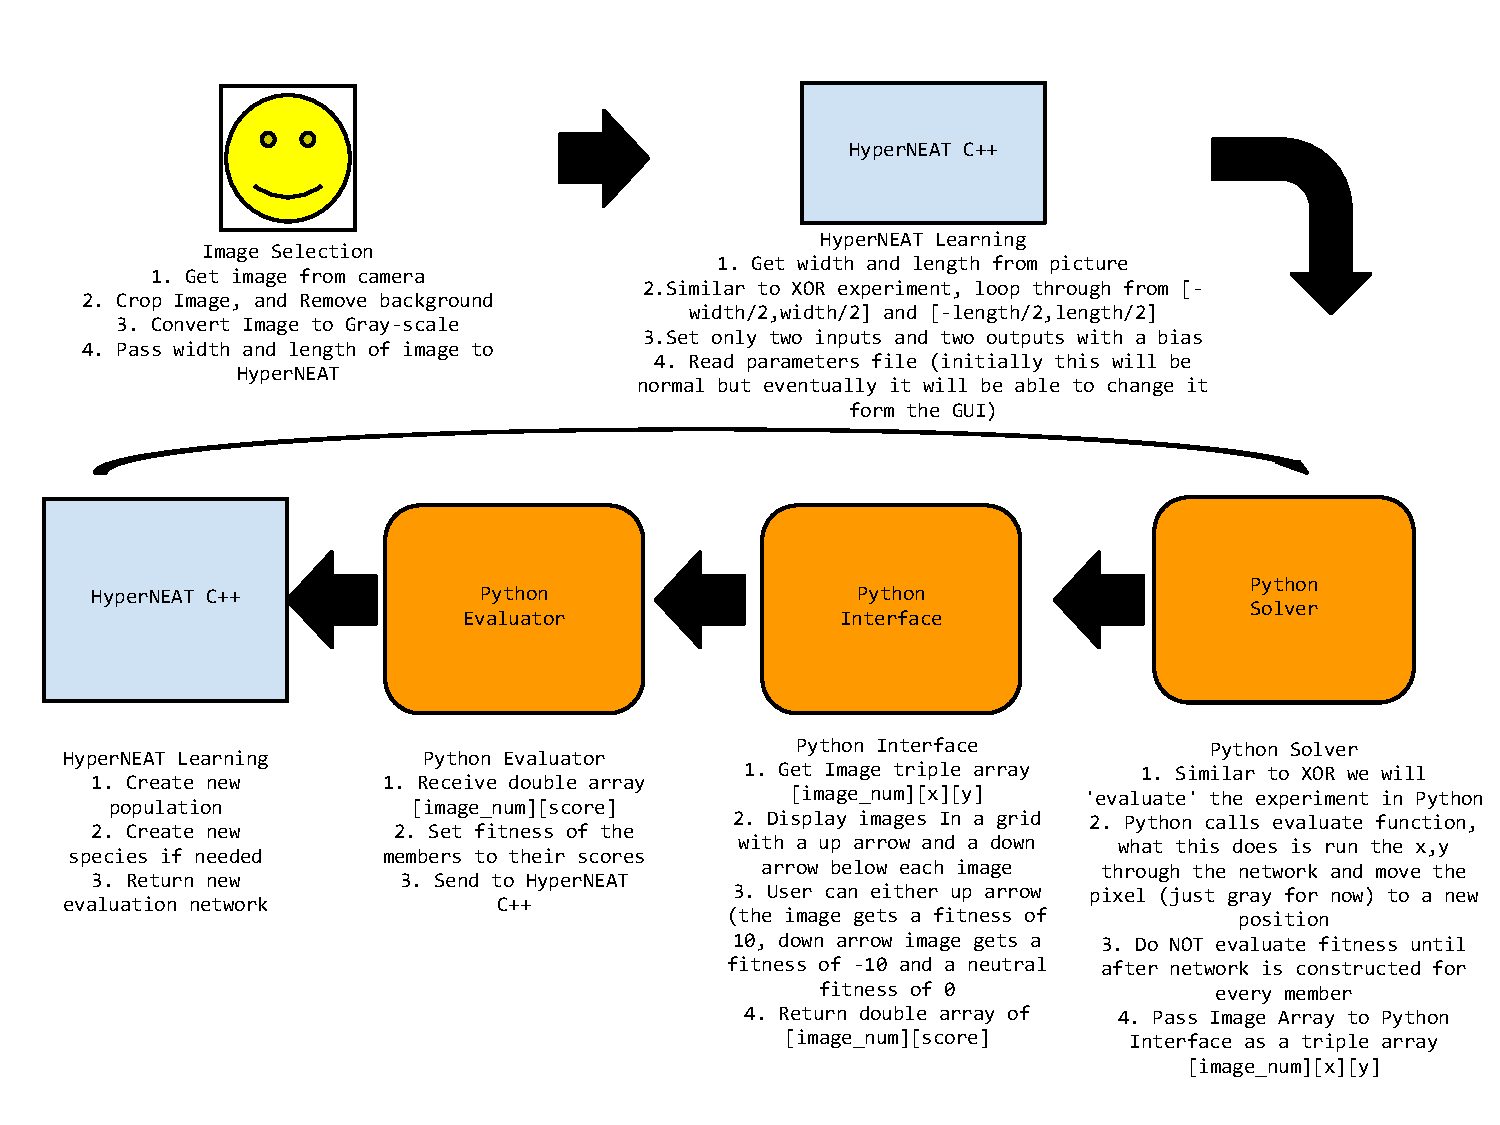
\includegraphics[width=\textwidth]{rec/arch.pdf}
%     \caption{Architecture}
%     \label{fig:arch}
% \end{figure}


As may be seen in figure \ref{fig:arch}, HyperNEAT C++ will be used
to manage the interal processing of the main HyperNEAT components
as that architecture already exists. However the Python system built
will be used to display the population (through a GUI built with Qt),
evaluate the viability of offspring (e.g. determine the fitness of
population individuals via operator input), and send the results back
to the HyperNEAT C++ layer for evolution.

An example of the GUI interface may be seen in figure \ref{fig:gui}.
This figure shows the general layout where a user will be able to
select an input image of a face and from there view and evolve the
resulting outputs. A network distortion rasterizer has been built
to utilize any given network representing a distortion in normalized
coordinates to determine a new image. In the figure some dummy networks
are shown which provide either a one to one pixel mapping or one or
two dimensional flipping as a proof of concept, but in general each
of the twelve figures would represent a different network that could
be selected by the user for evolution.

In addition to the display as shown, evolution parameters will be
avialable to the operator to change on the fly during evolution. The
useful parameters have not yet been determined which is why they do
not yet appear in the interface, but they will be added incrementally
as the need arises during testing.

Current progress to this effect includes a large overhaul of the Python
bindings available in the original HyperNEAT C++ code distribution
to allow for Python tests to be built, the development of a new experiment
module within HyperNEAT to support the necessary functionality, and
the development of a graphical user interface to allow operator interaction
with the evolutionary process. Most of the original work is presented
in the source section in \ref{sec:source}, though some minor changes
were omitted for brevity in this document.


\section{Questions}

Will image registration be required in order to generalize the evolved
structure to many different images from any angle? How do you define
the center of the picture, is it the nose feature’s centerpoint or
the centerpoint of the bounding box? Do the features of the face improve
the performance or detract? Should the evolved networks be seeded
with symmetry or can this be found efficiently? Can the facial features
be discovered and the neural network eventually understand the shapes
of evolved nose structures and eye structures? Will the neural network
allow for real time performance after evolution or should a transformation
matrix be calculated in order to utilize the evolved image transformations?


\section{Output}

Standalone GUI with image evolution capabilities, image saving capabilities
and neural network saving capabilities. This GUI will evolve a user’s
image and allow the user to view each individual generation.

As described in section \ref{sec:procedure}, the GUI in figure \ref{fig:gui}
is a representation of the operator interface.

\begin{figure}
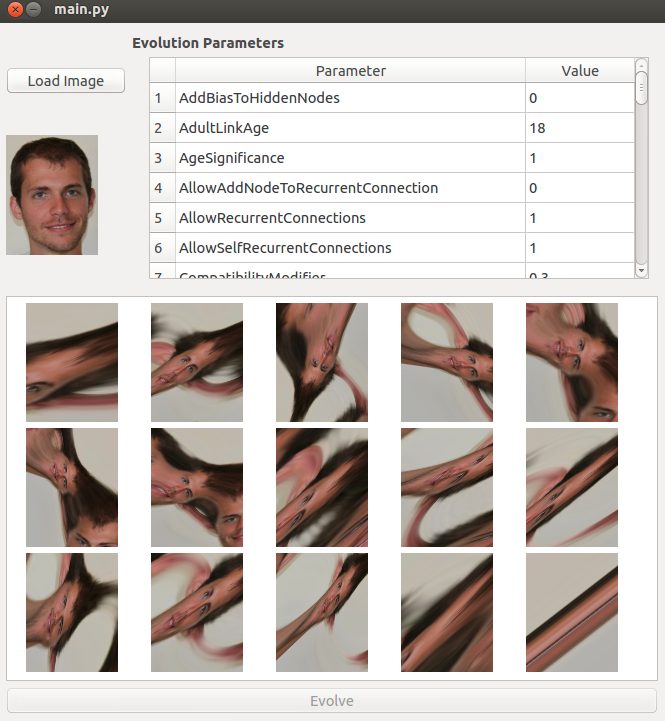
\includegraphics[width=1\textwidth]{rec/gui} \caption{GUI Prototype}


\label{fig:gui} 
\end{figure}



\section{Software}

HyperNeat v4.0 C++ by Jason Gauci, pyQt framework v4.2.8 for GUI representation,
OpenCV v 2.4, TinyXMLDLL v 2.0, JG template library, Boost C++, WxWidgets,
GCC, Cygwin (windows Dev), Ubuntu (Linux Dev), CMake,Make, Python
v 2.7


\section{Analysis}

\begin{figure}
\begin{centering}
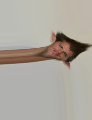
\includegraphics[scale=2]{rec/elfhead}
\par\end{centering}

\caption{``Pez elf head'' output}


\label{fig:common}
\end{figure}


As seen in \ref{fig:gui} the output of the current algorithm is extremely
noisy. Our current most seen output example can be best described
as a ``pez elf head'' transformation\ref{fig:common}. The CPNN
that produces this image is amazingly simple for such a complex transformation
\ref{fig:CPNN}, consisting of only three hidden nodes that only effect
the x-axis as expected. This image is so common amongst the output
of the algorithm that we are analyzing methods in order to increase
diversity within our evolved systems. It seems the biggest issue is
not the parameters but something more basic is how our approach is
modeled. We have observed the effect that when a user is evolving
images the number of generations usually does not extend past 50,
due in large part to the user quickly getting tired of picking images
individually to evolve and eventually decaying into a pseudo-random
type of search. This pseudo-random search makes it such that the CPNN's
quickly start to converge on an answer as the species start to mimic
each other in their genotype but vary in large ways with the phenotypes.
Ideally these phenotype variations would be good, but because most
of these phenotypes produce such a big distortion effect they are
unlikely to be chosen by the human for evolution and left on the cutting
room floor. 

It quickly becomes obvious what will happen in the situation described
above, because the slightest change to the genotype has a large impact
on the phenotype eventually those networks with larger variation will
be evolved out due to user selection. This forces a conformity across
the species with the phenotype expressed slightly differently e.g.
rotated along the y-axis as opposed to the x-axis. The conformity
eventually reaches endemic proportions with the all species reaching
a sort of minimization for what that user wants to observe based on
initial populations. In this situation the first random population
has a large effect on the final image. This represents a fundamental
change that must occur in future versions, that instead of a more
conservative approach either a novelty search or prior information
must be include in the algorithmic process. 

\begin{figure}
\begin{centering}
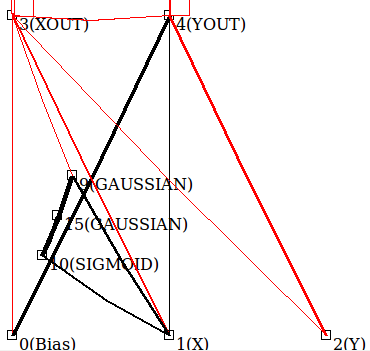
\includegraphics[width=1\textwidth]{rec/neuralnet}
\par\end{centering}

\caption{``Pez elf head'' CPNN }


\label{fig:CPNN}
\end{figure}



\section{Timeline and Work Distribution}
\begin{enumerate}
\item 9/12 - 9/24: Get build environment working between Windows and Ubuntu
(hyperNEAT and C++ bindings); use environment to build XOR using python.
Work Distribution: Independently get build working on respective platforms;
independently implement XOR. 
\item 9/24 - 9/28: Build initial project architecture modules: (1) the python/hyperNEAT
module that evolves CPPNs and sends the result to the user for evolution;
(2) python/GUI module that displays the results sent by module 1,
allows user selection, and returns the selection back to module 1
for further evolution. Work Distribution: Collaboratively determine
python interface between modules; independently build first pass of
respective modules; collaboratively work on implementation. 
\item 9/28 - 10/3: Independently compile necessary documentation and graphics
for respective modules; collaboratively compile documentation linking
the two and considering the overall system architecture. 
\item 10/3 - 10/24: Experiment with evolution to attempt to evolve an interesting
deformation (independently); through experimentation work out any
software bugs; this is the baseline project implementation. 
\item 10/24 - 10/29: Consolidate interesting findings, issues, and experiences
into the midterm report and presentation. 
\item 10/29 - 11/26: Use time as buffer to finish work on the baseline if
good results weren’t obtained. If acceptable results were found, attempt
to increase applicability and complexity by looking at extensions
including: detecting image features to be used in the transform instead
of just pixel locations; integrating evolved neural nets in a video
(real time). 
\item 10/26 - 10/29: Complete Midterm report and Midterm Presentation. 
\item 10/30 - 11/10: Implement ``Haar Cascades'' to detect facial features.
These facial features will be the only ones evolved. The facial features
will take the place of the whole image and instead of evolving everything
on the image including head position we will just evolve these individual
features.
\item 11/11 - 11/26: Collect images, videos and perform basic statistical
analysis on the outputs. Perform a basic user study and develop an
outline for the final paper and presentation. Write up analysis about
project and discussion sections for final paper.
\item 11/27 - 12/2: Finish Final presentation and final paper.
\item 12/2 - 12/7: Complete final paper.
\end{enumerate}

\section{Source Code}

\label{sec:source}


\subsection{PyHyperNEAT.cpp}

\lstinputlisting{[}language=C++{]}{../../external/HyperNEAT/NE/HyperNEAT/PyHyperNEAT/src/PyHyperNEAT.cpp}

%\subsection{HCUBE\_ExperimentRun.cpp}
%\lstinputlisting[language=C++]{../external/HyperNEAT/NE/HyperNEAT/HyperCube_NEAT/src/HCUBE_ExperimentRun.cpp}



\subsection{ImageExperiment.h}

\lstinputlisting{[}language=C++{]}{../../src/hyperneat/ImageExperiment/ImageExperiment.h}


\subsection{ImageExperiment.cpp}

\lstinputlisting{[}language=C++{]}{../../src/hyperneat/ImageExperiment/ImageExperiment.cpp}


\subsection{GUIWindow.py}

\lstinputlisting{[}language=Python{]}{../../src/gui/GUIWindow.py}


\subsection{PopulationModel.py}

\lstinputlisting{[}language=Python{]}{../../src/gui/PopulationModel.py}
\end{document}
